\documentclass[conference]{IEEEtran}
\usepackage[T1]{fontenc}
\usepackage{cite}
\usepackage{amsmath}
\usepackage{graphicx}
\usepackage{booktabs}
\usepackage{multirow}
\usepackage{url}
\usepackage{xcolor}
\graphicspath{{figures/}}
\newcommand{\up}{$^{+}$}
\newcommand{\dn}{$^{-}$}

\begin{document}

\title{Latent Profiles for Oblique Retrieval:\\Document-Side LLM Descriptions on OBLIQ-Bench}

% TODO: fill in author name(s), roll number(s) and e-mail.
\author{\IEEEauthorblockN{Author Name}
\IEEEauthorblockA{IT550 Information Retrieval (Prof.\ Sandip Modha)\\
Institute name\\
email@example.com}}

\maketitle

\begin{abstract}
Oblique queries are relevant through a hidden property of the document, such as a proof technique or an author's style, rather than its topic. OBLIQ-Bench showed that modern retrievers handle them poorly and tried only query-side fixes; its GPT-5.2 query rewriter collapsed Writing-Style from nDCG@10 0.164 to 0.018. We test the document side instead. An open LLM (Qwen2.5-7B-Instruct) reads every document once, offline, and writes a short \emph{latent profile} of its hidden traits. Profiles are indexed with BM25 and Qwen3-Embedding-0.6B beside the raw text, and the four ranked lists are fused with reciprocal rank fusion. On Math, the fused system lifts pooled nDCG@10 from 0.147 to 0.175, above the paper's best single-stage retriever (Gemini-2-Embedding, 0.147), and beats the text baseline on held-out queries ($p=0.023$ gold, $0.013$ pooled). It also beats the same LLM used as a query rewriter. On Writing-Style the method fails (0.060 vs.\ 0.099 for BM25): profiles carry almost no author signal (same- vs.\ different-author AUC 0.55), while character n-grams and a style embedding do (fused, 0.128). Ablations show that profiler size matters (3B is significantly worse than 7B) while profile length and the no-topic instruction do not, and a 7B listwise re-ranker hurts. All experiments use open models and about six GPU-hours on free Kaggle T4s.
\end{abstract}

\begin{IEEEkeywords}
information retrieval, document expansion, large language models, rank fusion, authorship, mathematical retrieval
\end{IEEEkeywords}

%=====================================================================
\section{Introduction}

Modern retrievers match topics well and hidden properties badly. A query such as ``find other problems solved by the same telescoping trick'' or ``find more writing by this author'' shares few words, and often no topic, with its relevant documents. OBLIQ-Bench~\cite{obliq2026} calls these \emph{oblique queries} and shows that every retriever it tests scores low on them: the best single-stage system, Gemini-2-Embedding, reaches nDCG@10 of 0.147 on Math and 0.164 on Writing-Style.

The paper tries two query-side fixes with GPT-5.2: rewriting the query once, and a four-round multi-hop agent. Both help on Math (0.185, 0.207), but the rewriter collapses Writing-Style to 0.018 because the rewritten query drifts back to the topic. The paper names the document side as an open direction.

We take that direction. A small open LLM reads each document once, offline, and writes a \emph{latent profile}: a short, fixed-format description of hidden traits (the proof move, the author's habits), with an explicit instruction not to mention the topic. Profiles are indexed beside the raw text, each query is profiled with the same prompt, and the ranked lists are fused. The idea extends Doc2Query~\cite{doc2query} from predicted queries to predicted hidden properties. We ask:
\begin{itemize}
\item \textbf{RQ1} Can we reproduce the paper's BM25 and Qwen3-Embedding-0.6B numbers?
\item \textbf{RQ2} Do profiles alone beat raw text?
\item \textbf{RQ3} Does fusing text and profiles beat either alone?
\item \textbf{RQ4} Does document-side profiling beat query-side rewriting with the same LLM?
\item \textbf{RQ5} How much of the gap to the paper's oracle re-ranker does a small open re-ranker close?
\end{itemize}

Our contributions are: (i) a document-side method that uses only open models and free compute; (ii) on Math, a significant gain over the text baseline that passes the paper's best single-stage score; (iii) on Writing-Style, a careful negative result with an analysis of why profiles miss authorship, plus non-LLM style baselines showing the signal exists; and (iv) a same-LLM comparison with query rewriting, and ablations of profiler size, profile length and the no-topic rule.

%=====================================================================
\section{Related Work}

\textbf{Oblique and reasoning-intensive retrieval.} OBLIQ-Bench~\cite{obliq2026} is our base: five tasks where relevance rests on a latent property, with query-side baselines and an oracle re-ranker given the gold document. BRIGHT~\cite{bright} also targets retrieval that needs reasoning. Weller et al.~\cite{weller2026} prove limits on what single-vector embeddings can represent, one reason to add a second, differently built index rather than a better embedder.

\textbf{Document expansion.} Doc2Query~\cite{doc2query} appends predicted queries to each document; Doc2Query-{}-~\cite{doc2queryminus} filters out expansions that drift off the document. Our profiles are a document expansion that describes hidden traits instead of likely queries, kept in its own index rather than appended to the text.

\textbf{Query-side LLM expansion.} HyDE~\cite{hyde} and Query2doc~\cite{query2doc} let an LLM write a pseudo-document from the query. OBLIQ-Bench's rewriter is of this kind, and its Writing-Style collapse is the failure we try to avoid by working on the documents.

\textbf{LLM re-ranking and fusion.} RankGPT~\cite{rankgpt} re-ranks with sliding-window listwise prompts; our E5 uses that scheme with a 7B open model. Reciprocal rank fusion~\cite{rrf} combines ranked lists without score calibration, which suits indexes as different as BM25 over profiles and dense vectors over text.

\textbf{Authorship representations.} LUAR~\cite{luar} and the Style-Embedding model of Wegmann et al.~\cite{wegmann2022} learn author or style vectors from many texts per author. We use the latter, with character n-gram TF-IDF, as non-LLM baselines on Writing-Style.

%=====================================================================
\section{Method}

The method adds one offline step, profiling, and one LLM call per query at search time (Fig.~\ref{fig:pipeline}).

\begin{figure*}[t]
\centering
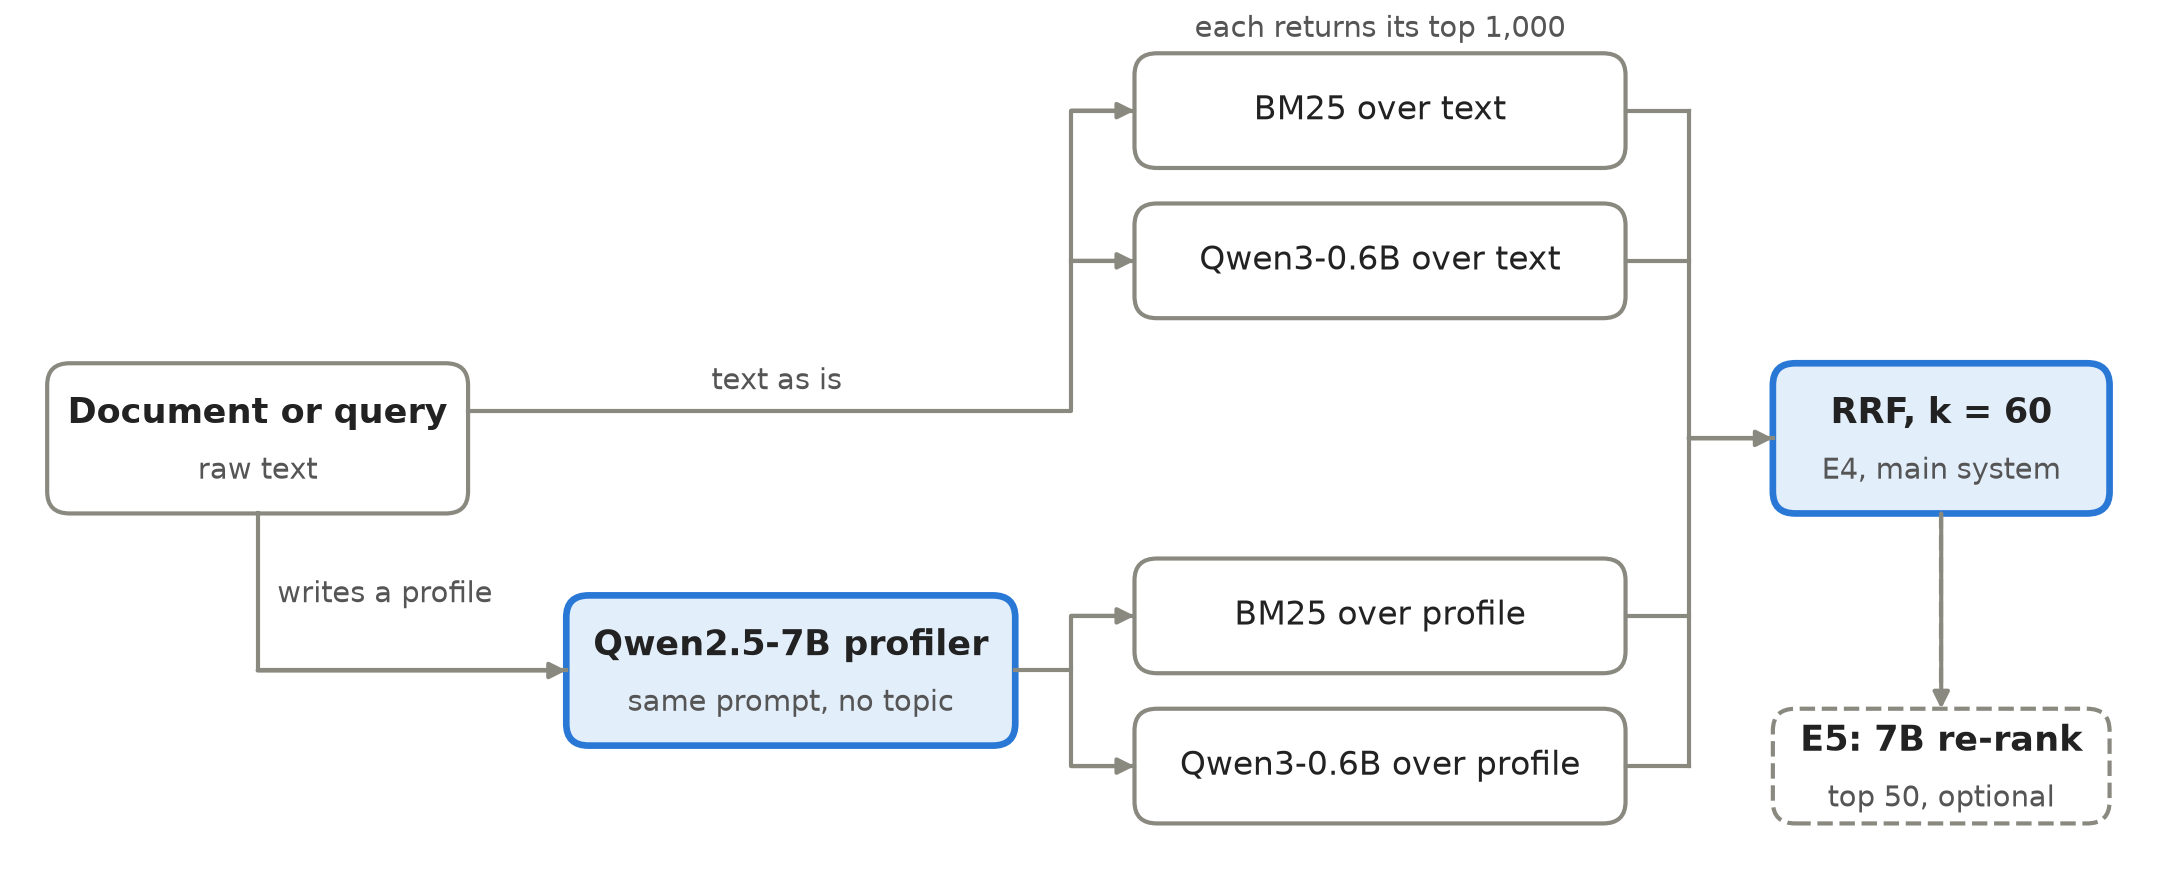
\includegraphics[width=0.82\textwidth]{fig0_pipeline.png}
\caption{Pipeline. Documents are profiled once, offline; each query is profiled once at search time with the same prompt. Four indexes each return their top 1,000, and RRF fuses them (E4). E5 optionally re-ranks the top 50.}
\label{fig:pipeline}
\end{figure*}

\subsection{Latent profiles}
Qwen2.5-7B-Instruct~\cite{qwen25} (AWQ 4-bit, served with vLLM~\cite{vllm}) reads each document and writes a 60--100-word profile in a fixed, labelled format, with greedy decoding and frequency penalty 0.3. The core instruction is to describe the hidden trait and \emph{not} the topic. One prompt per task is used for both documents and queries.
\begin{itemize}
\item \textbf{Math}: ``Do not solve it in full. Work out the core reasoning move a solution needs \ldots{} Name reasoning techniques, not the topic. Do NOT mention the field or the objects involved.'' Fields: Techniques, Proof move (3--5 abstract steps), Key insight, Also known as; words only, no formulas.
\item \textbf{Writing}: ``You are a stylometry expert. Describe what makes the AUTHOR of the passage recognisable, so that the same author could be identified from a passage on a completely different topic \ldots{} Do NOT mention the subject matter.'' Fields: Voice, Sentences, Punctuation, Tone and humour, Signature phrases, Other habits.
\end{itemize}
Both prompts were frozen after two rounds of hand-testing on 20 documents per task.

\subsection{Indexes and fusion}
We build four indexes: BM25~\cite{bm25} and Qwen3-Embedding-0.6B~\cite{qwen3emb} over raw text, and the same two over profiles. BM25 is \texttt{rank-bm25} with default parameters, as in the paper; dense search is exact inner product in FAISS. The main system (E4) fuses the four top-1,000 lists with reciprocal rank fusion:
\begin{equation}
\mathrm{RRF}(d)=\sum_{i=1}^{4}\frac{w_i}{k+\mathrm{rank}_i(d)},\qquad k=60,
\end{equation}
with equal weights $w_i=1$. We also report weights tuned on the dev split.

\subsection{Baselines and variants}
\textbf{E2, query rewriting:} the same 7B model rewrites each query once, and the rewrite is searched with Qwen3 over raw text. On Writing we use the paper's authorship rewriter prompt verbatim; the paper gives no Math rewriter prompt, so ours follows its published Twitter template.
\textbf{E3:} RRF of the two profile indexes only.
\textbf{E5, re-ranking:} the 7B model re-ranks the top 50 of E4 with a RankGPT-style listwise prompt (window 20, step 10). Unlike the paper's oracle, no gold document is injected.

%=====================================================================
\section{Experimental Setup}

\begin{table}[t]
\centering
\caption{Tasks used (from OBLIQ-Bench).}
\label{tab:data}
\footnotesize
\begin{tabular}{@{}lrrrl@{}}
\toprule
Task & Queries & Corpus & Rel./query & Labels \\
\midrule
Math Meta-Program & 151 & 3,508 & 13.5 / 14.3 & GPT-5, clustered \\
Writing-Style & 512 & 10,389 & 9.0 & authorship (62 authors) \\
\bottomrule
\end{tabular}
\\[2pt]{\scriptsize Rel./query: Math gold / pooled; Writing gold.}
\end{table}

\textbf{Data.} Table~\ref{tab:data} summarises the two tasks. A Math query asks for problems that share the core reasoning of a given problem; the corpus holds problem statements only. A Writing query is a blog snippet, and the relevant documents are other snippets by the same author.

\textbf{Exclusion mask.} Each task ships \texttt{per\_query\_excluded\_ids.json}; on Writing it hides snippets from the same source post. Every run passes through a single mask function before scoring, and the evaluator refuses unmasked runs.

\textbf{Metrics.} nDCG@10 is the main metric, with nDCG@50 and Recall@10/50/100, computed with ranx~\cite{ranx}. Math is scored with gold and pooled judgments; pooled judgments came from the paper's systems and can under-score a new system that finds unjudged relevant documents.

\textbf{Dev/test split and significance.} A fixed 20\% of queries (seed 0) forms the dev split: 30 Math and 102 Writing queries. Every choice (BM25 tokenizer, dense query prompt, fusion weights) is made on dev. We report all queries and the 80\% test split, and claim a win only when a paired $t$-test on test nDCG@10 gives $p<0.05$.

\textbf{Compute.} LLM profiling, rewriting and re-ranking run on Kaggle (2$\times$ Tesla T4). Dense encoding runs on a laptop RTX~4050 (6\,GB); BM25, fusion and evaluation run on its CPU. Every LLM output is cached to disk and generated exactly once.

%=====================================================================
\section{Results}

All numbers are masked; Math cells read gold/pooled.

\subsection{Reproduction (RQ1)}
Both baselines reproduce (Table~\ref{tab:e1}). Qwen3-0.6B lands within 0.005 of the paper on every metric of both tasks. Our BM25 is slightly stronger than the paper's (up to +0.017), the conservative side for our claims; no single BM25 tokenizer matches both tasks. In the systems that follow, text components use the tokenizer and prompt picked on dev.

\begin{table}[t]
\centering
\caption{E1 reproduction: ours (paper in brackets).}
\label{tab:e1}
\footnotesize
\begin{tabular}{@{}lll@{}}
\toprule
System & nDCG@10 & R@100 \\
\midrule
Math BM25 & .028/.035 (.022/.029) & .089/.095 (.088/.029) \\
Math Qwen3-0.6B & .115/.142 (--/.143) & .309/.336 (.309/.336) \\
Writing BM25 & .083 (.077) & .225 (.208) \\
Writing Qwen3-0.6B & .045 (.046) & .107 (.103) \\
\bottomrule
\end{tabular}
\\[2pt]{\scriptsize Some paper Math BM25 pooled cells look like typos (R@50 = R@100 = .029). TODO: fill the paper's Math Qwen3 gold nDCG@10.}
\end{table}

\begin{table*}[t]
\centering
\caption{Main results. nDCG@10 and Recall@100 on all queries; $p$ = paired $t$-test on test nDCG@10 vs.\ the best E1 baseline picked on dev (Math: Qwen3 text; Writing: BM25 text), with $^{+}$/$^{-}$ = better/worse on average. Bold: main system.}
\label{tab:main}
\footnotesize
\begin{tabular}{@{}lccccccc@{}}
\toprule
& \multicolumn{3}{c}{Math (gold/pooled)} && \multicolumn{3}{c}{Writing-Style (gold)} \\
\cmidrule{2-4}\cmidrule{6-8}
System & nDCG@10 & R@100 & $p$ (test) && nDCG@10 & R@100 & $p$ (test) \\
\midrule
BM25 text (E1) & .060/.072 & .178/.188 & 7e-5\dn/4e-6\dn && .099 & .245 & baseline \\
Qwen3-0.6B text (E1) & .117/.147 & .313/.341 & baseline && .045 & .107 & 2e-15\dn \\
E2: 7B query rewrite + Qwen3 & .104/.141 & .341/.366 & .64/.83 && .023 & .075 & 2e-25\dn \\
E3: profiles only & .124/.146 & .368/.382 & .35/.74 && .010 & .058 & 1e-29\dn \\
\textbf{E4: text + profiles, RRF} & \textbf{.142/.175} & .383/.410 & \textbf{.023\up/.013\up} && .060 & .196 & 5e-9\dn \\
E4, dev-tuned weights & .162/.195 & .439/.456 & 9e-4\up/4e-4\up && .098 & .252 & .45 \\
E5: E4 + 7B listwise re-rank & .126/.156 & .383/.410 & .19/.23 && -- & -- & -- \\
E4, solution-aware profiles$^\dagger$ & .144/.174 & .437/.459 & .008\up/.007\up && -- & -- & -- \\
E4, profiles w/o Voice/Tone & -- & -- & -- && .075 & .205 & 6e-6\dn \\
Char 3--5-gram TF-IDF$^\ddagger$ & -- & -- & -- && .091 & .266 & .19 \\
Style-Embedding$^\ddagger$ & -- & -- & -- && .075 & .210 & .019\dn \\
BM25 + char n-gram + Style-Emb.$^\ddagger$ & -- & -- & -- && .128 & .353 & 6e-9\up \\
\midrule
\multicolumn{8}{@{}l}{\emph{Paper (nDCG@10; Math pooled):} Gemini-2-Embedding .147 / .164; GPT-5.2 rewriter + Gemini .185 / .018; multi-hop agent .207 / .061; oracle re-ranker .329 / .515} \\
\bottomrule
\end{tabular}
\\[2pt]{\scriptsize $^\dagger$Documents profiled together with their solutions, which the paper's retrievers never saw; not a headline number. $^\ddagger$Non-LLM style baselines, not part of the profile method.}
\end{table*}

\begin{figure*}[t]
\centering
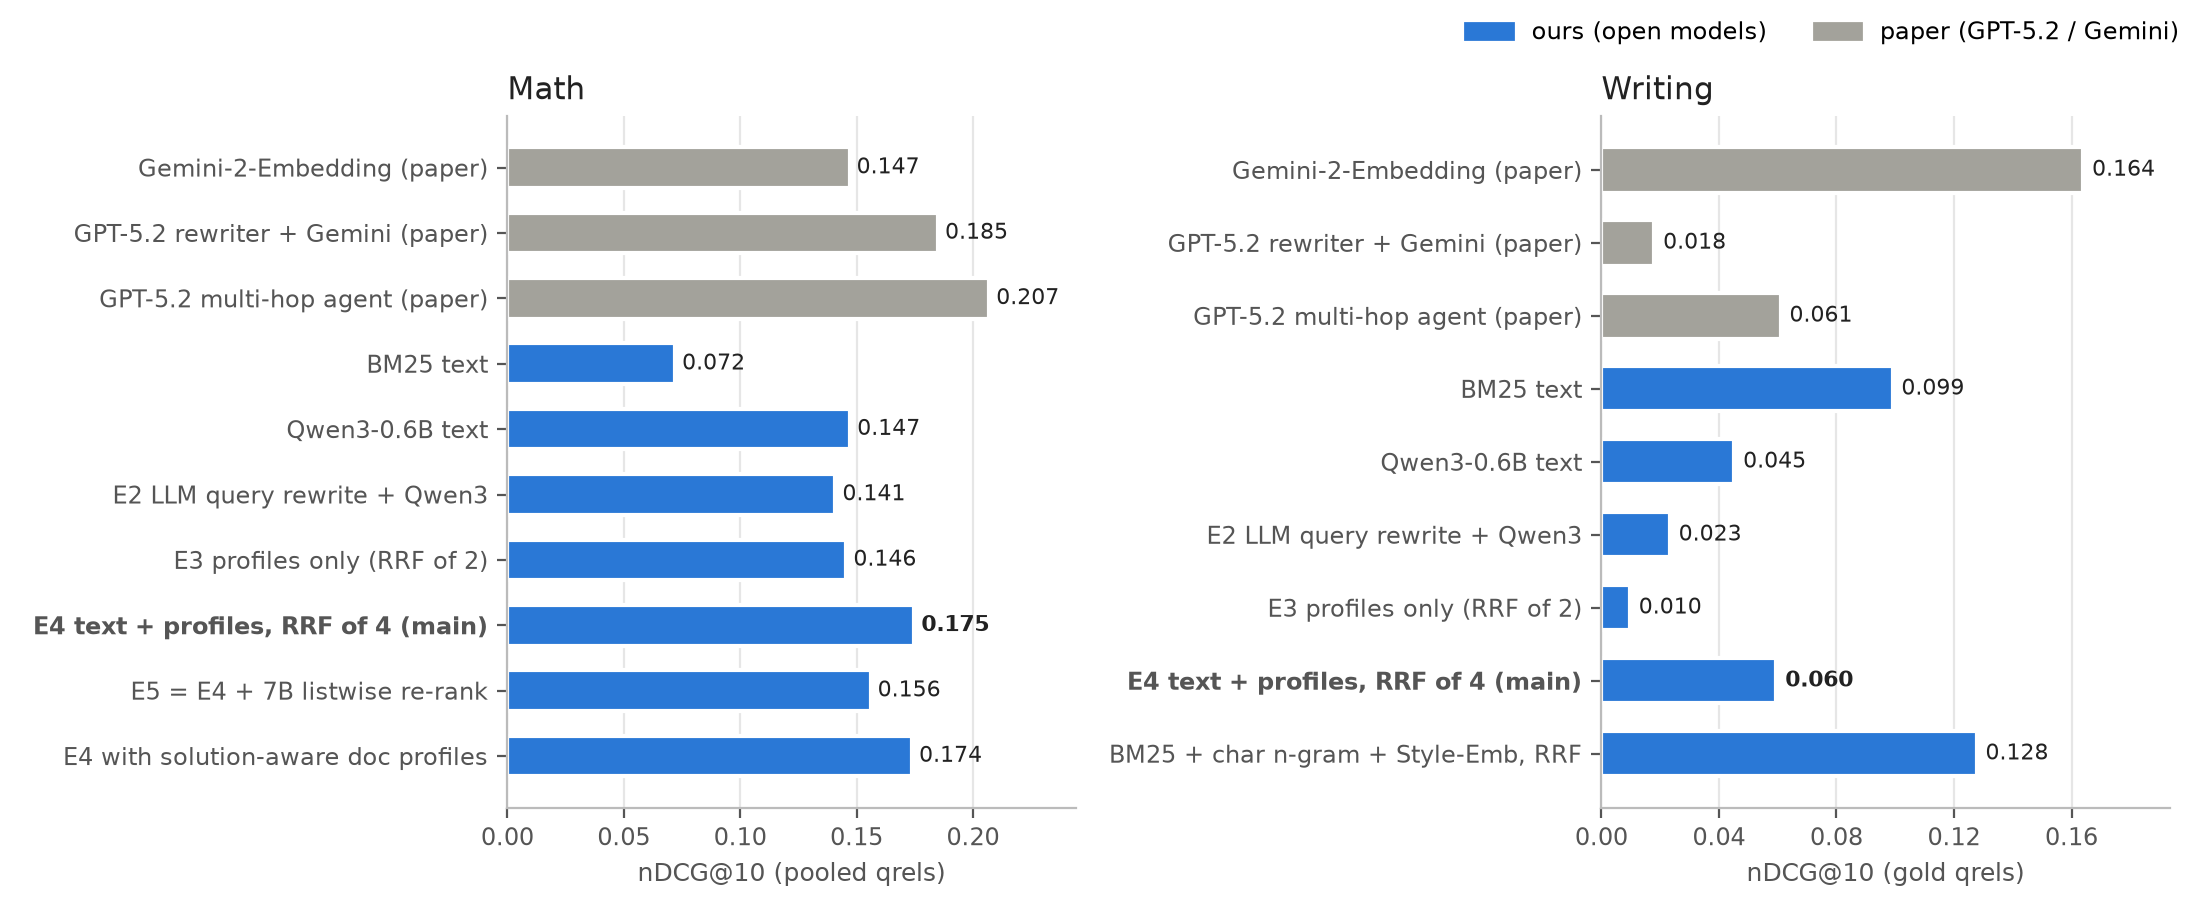
\includegraphics[width=\textwidth]{fig1_main_results.png}
\caption{nDCG@10 of our systems (blue) and the paper's (grey). Math uses pooled judgments, as the paper's headline does; the oracle re-ranker is omitted because it is given the gold document.}
\label{fig:main}
\end{figure*}

\subsection{Math (RQ2--RQ5)}
E4 reaches 0.175 pooled nDCG@10, above the paper's Gemini-2-Embedding (0.147), and beats the Qwen3 text baseline on test queries ($p=0.023$/$0.013$; Table~\ref{tab:main}, Fig.~\ref{fig:main}).
\textbf{RQ2:} profiles alone (E3) match the text baseline (0.146 vs.\ 0.147 pooled, not significant) without using the problem text at query time.
\textbf{RQ3:} fusion beats both. Fusing the two \emph{text} indexes alone gives 0.098/0.124, below Qwen3 text, so the gain comes from the profiles rather than from fusing more lists.
\textbf{RQ4:} E4 beats the same LLM used as a query rewriter ($p=0.012$/$0.029$ on test); E2 itself is no different from Qwen3 text.
\textbf{RQ5:} the 7B re-ranker makes E4 worse (0.156 vs.\ 0.175 pooled; 46 queries worse, 23 better) and closes none of the gap to the oracle's 0.329.
Weights tuned on the 30 dev queries ($[0, 2, 0.5, 0.5]$, dropping BM25 text) reach 0.197 pooled on test, above the paper's GPT-5.2 rewriter (0.185). We keep equal-weight E4 as the headline because 30 queries is a small basis for tuning.

\subsection{Writing-Style (RQ2--RQ4)}
Profiles fail on Writing. E4 (0.060) is significantly \emph{below} BM25 over raw text (0.099), and profiles alone score 0.010. Dropping the templated Voice and Tone fields, or keeping only Signature phrases and Other habits, makes profiles worse (0.004--0.006 alone). RQ4 still holds: the rewriter reproduces the paper's collapse with an open LLM (0.023, half of Qwen3 on the original query, $p=4\times10^{-7}$), and E4 beats it ($p=2\times10^{-12}$). The style signal does exist: character n-grams and a style embedding each match BM25 alone, and their fusion with BM25 reaches 0.128 ($p=6\times10^{-9}$), still below Gemini's 0.164. Adding the profile indexes to that fusion lowers it to 0.110.

\subsection{Ablations}
Profiler size matters; length and the no-topic rule do not (Table~\ref{tab:abl}). Each variant re-profiles all of Math and plugs into the main system's components unchanged. Only A2's profiles-only score differs significantly from the main system ($p=0.008$/$0.006$); no E4 difference is significant. The A1 instruction raised the topic-word rate only from 42\% to 48\%, so it is a weak test of the no-topic rule: the 7B model mixes in topic words either way.

\begin{table}[t]
\centering
\caption{Math ablations (nDCG@10, gold/pooled). Topic = share of document profiles using a banned example word (triangle, polynomial, matrix, prime, graph, integral, sequence).}
\label{tab:abl}
\footnotesize
\begin{tabular}{@{}lcccc@{}}
\toprule
Profiles & Words & Topic & E3 & E4 \\
\midrule
Main: 7B, no topic, 60--100 w. & 59 & 42\% & .124/.146 & .142/.175 \\
A1: topic words allowed & 61 & 48\% & .116/.147 & .142/.178 \\
A2: 3B profiler & 55 & 40\% & \textbf{.091/.108} & .128/.149 \\
A3: $\sim$40-word profiles & 43 & 35\% & .120/.136 & .138/.169 \\
\bottomrule
\end{tabular}
\\[2pt]{\scriptsize Bold: significantly below main on test ($p<0.01$). All other differences $p>0.09$.}
\end{table}

\subsection{Cost}
One-off profiling costs 16 GPU-minutes for Math and 158 for Writing (Table~\ref{tab:cost}). Online, E4 costs about 100\,ms per query on a laptop CPU (BM25 57\,ms, profile BM25 38\,ms, two FAISS searches and RRF under 4\,ms), plus one LLM call of about 100 output tokens to profile the query. E5 adds about 18 GPU-seconds per query.

\begin{table}[t]
\centering
\caption{One-off LLM cost on Kaggle (2$\times$ T4).}
\label{tab:cost}
\footnotesize
\begin{tabular}{@{}lrr@{}}
\toprule
Job & Items & GPU-min \\
\midrule
Writing profiles, 7B (main) & 10,484 & 158 \\
Math profiles with solutions (variant) & 3,493 & 71 \\
E5 re-rank, Math top 50 & 604 windows & 45 \\
Math profiles, topic allowed (A1) & 3,659 & 21 \\
Math profiles, 7B (main) & 3,639 & 16 \\
Math profiles, $\sim$40 words (A3) & 3,659 & 16 \\
Math profiles, 3B (A2) & 3,659 & 13 \\
Query rewrites (E2), Writing / Math & 512 / 151 & 13 / 7 \\
\bottomrule
\end{tabular}
\end{table}

%=====================================================================
\section{Analysis}

\subsection{Where profiles help and hurt on Math}
Profiles help when they name a specific move and hurt when the move is generic. Per query, E4 beats Qwen3 text on 59 queries, loses on 35 and ties on 57, mostly where both score 0 (Fig.~\ref{fig:scatter}).

\textbf{Helped.} Query q01094 asks for a closed form of $\sum_n 4^n\sin^4(2^{-n}\theta)$. Its profile reads ``Recognize a trig identity $\rightarrow$ Simplify the sine term $\rightarrow$ Transform the series into a telescoping form $\rightarrow$ Sum the series''. A relevant problem profiled as ``Identify a telescoping series $\rightarrow$ Simplify each term using trigonometric identities \ldots'' rises from rank 77 under Qwen3 text to rank 1 (nDCG@10 0.28 $\rightarrow$ 0.63). Likewise, block-determinant structure lifts q01890 from 0.00 to 0.40, and an Implicit Function Theorem plus Jacobian-rank check lifts a relevant problem for q02887 from rank 24 to 2. Profiles turn different-looking problems into near-identical descriptions of the same move.

\textbf{Hurt.} The worst losses are series-evaluation problems with generic profiles, e.g.\ ``Series manipulation, zeta function properties, Euler product'' (q01549). Many problems receive near-identical profiles of this kind and crowd out a gold document that Qwen3 text ranked first; it falls to rank 33 (0.54 $\rightarrow$ 0.17). Contour-integration problems fail the same way.

\textbf{Topic leakage.} Profiles still name determinants, sine terms and the zeta function despite the instruction; 42\% use a banned example word. Ablation A1 suggests this leak costs little.

\begin{figure}[t]
\centering
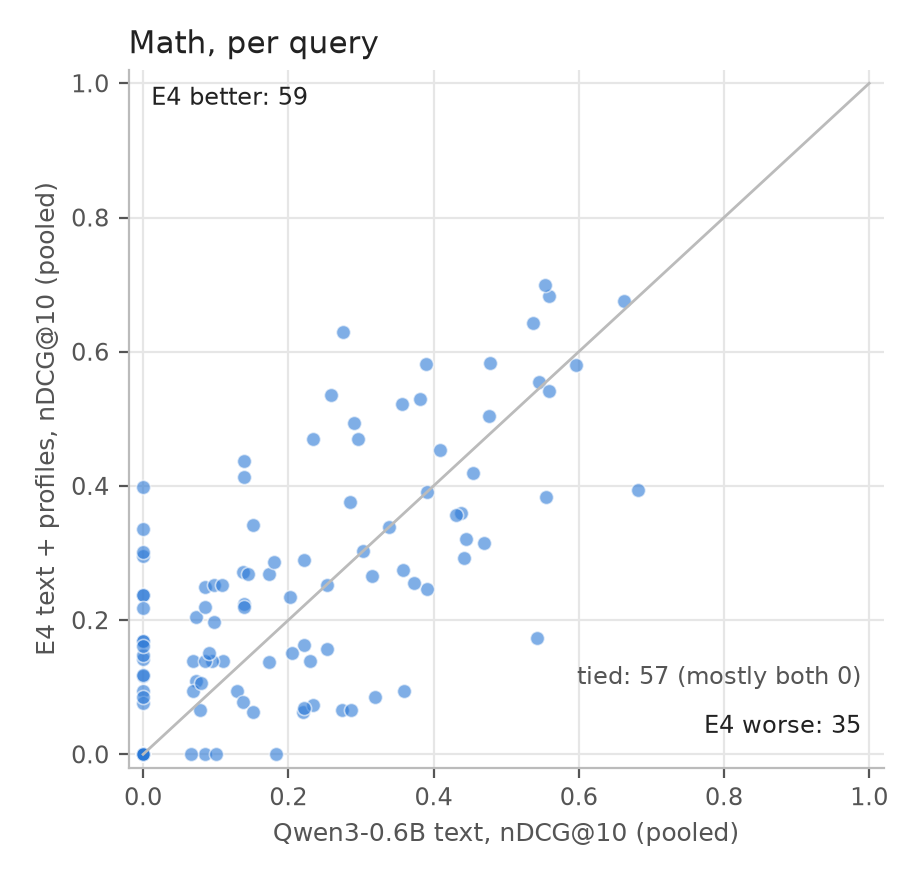
\includegraphics[width=0.9\columnwidth]{fig3_per_query_math.png}
\caption{Math, per-query pooled nDCG@10: Qwen3-0.6B text vs.\ E4. Points above the diagonal are queries E4 improves.}
\label{fig:scatter}
\end{figure}

\subsection{Why profiles fail on Writing}
The profiles describe blog writing in general, not the author. First, output is templated: 36\% of document profiles share the exact Voice line ``we, neutral and informative, formal'', and the Signature-phrases field mostly quotes topical phrases. Second, profiles carry no author signal. On the 540 author-labelled snippets (62 authors, same-post pairs removed) we measure the AUC of same- vs.\ different-author cosine similarity (Table~\ref{tab:auc}, Fig.~\ref{fig:hist}). Every profile variant sits near chance, while three raw-text representations separate authors. Raw Qwen3 scoring highest is likely topic rather than style, since an author tends to write about the same subjects.

A 7B model asked to describe style falls back on generic register words that every blog shares, while what tells authors apart is low-level and frequent: character sequences, function words, punctuation. A prompt cannot easily make the model count those; an encoder trained for authorship already does.

\begin{table}[t]
\centering
\caption{Writing: same- vs.\ different-author similarity (AUC; 0.5 = chance).}
\label{tab:auc}
\footnotesize
\begin{tabular}{@{}lccc@{}}
\toprule
Representation & cos same & cos diff & AUC \\
\midrule
Profile, all fields (Qwen3) & .713 & .699 & .550 \\
Profile, no Voice/Tone & .703 & .690 & .546 \\
Profile, Signature + Habits & .597 & .584 & .538 \\
Raw text, char 2--4-gram TF-IDF & .197 & .175 & .645 \\
Raw text, Style-Embedding & .786 & .654 & .654 \\
Raw text, Qwen3-0.6B & .265 & .207 & .663 \\
\bottomrule
\end{tabular}
\end{table}

\begin{figure*}[t]
\centering
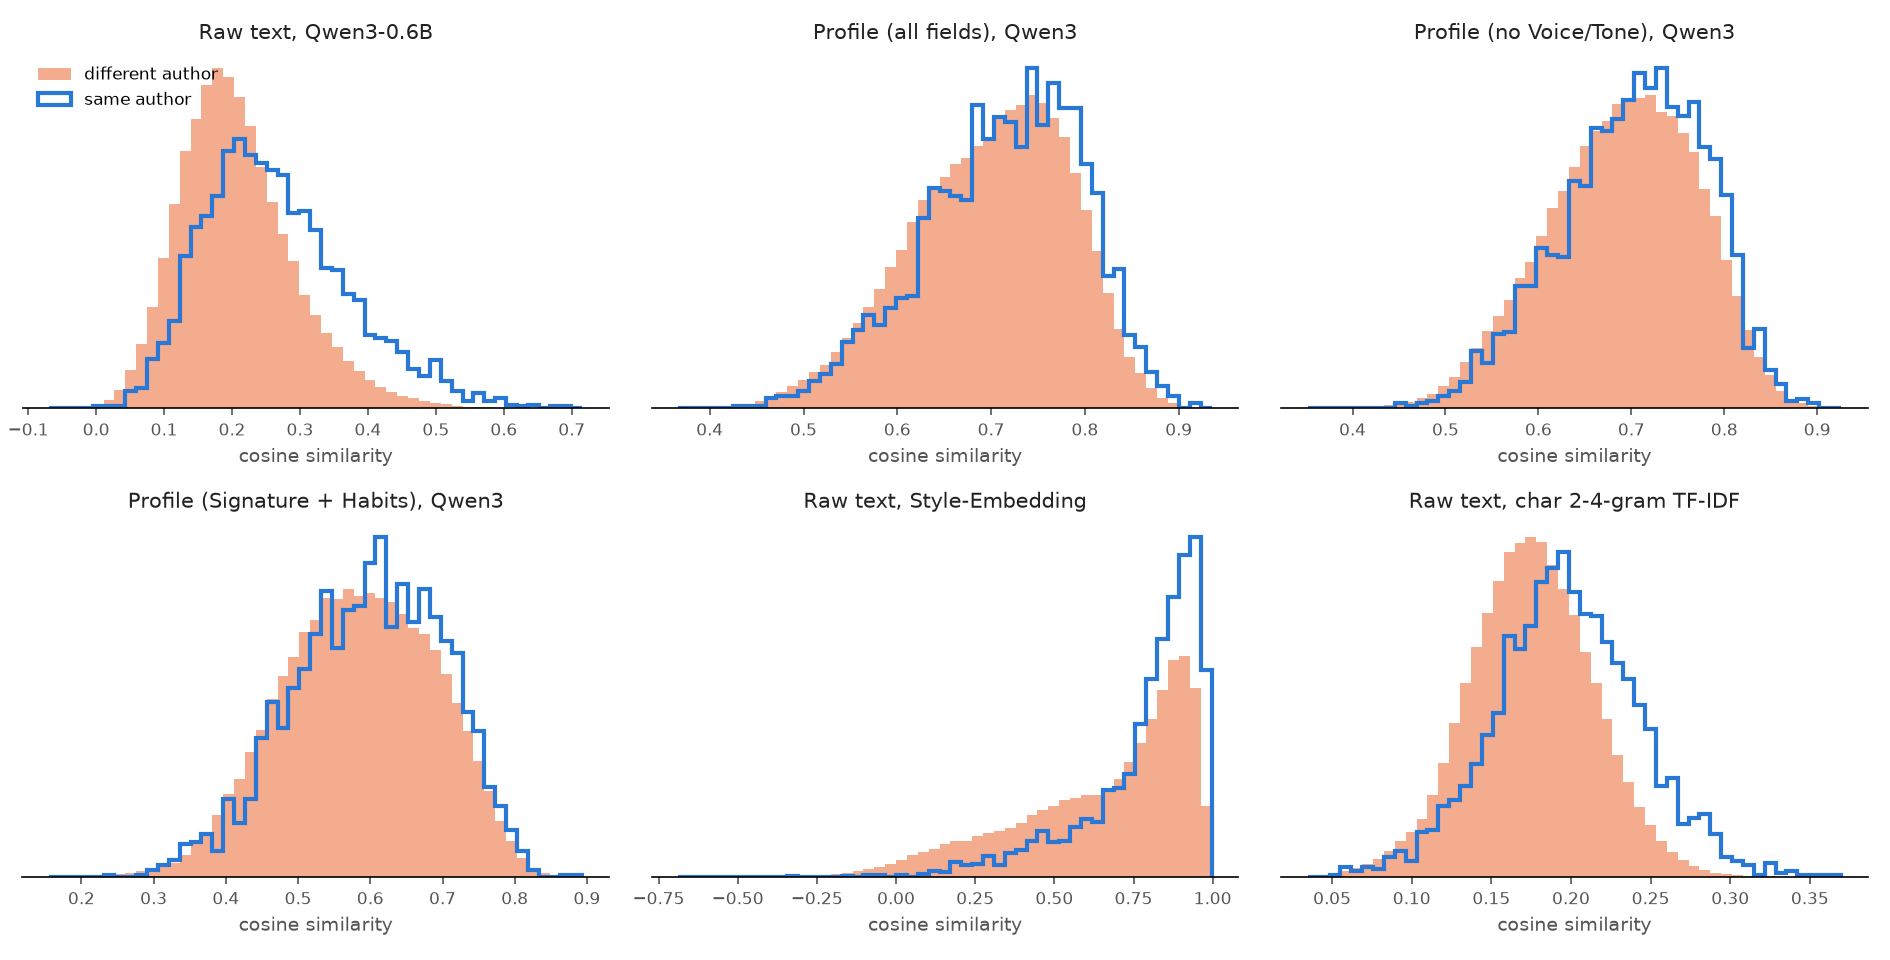
\includegraphics[width=0.9\textwidth]{fig4_writing_author_similarity.png}
\caption{Writing: cosine similarity of same-author (blue line) and different-author (orange fill) snippet pairs. Profile panels overlap almost completely.}
\label{fig:hist}
\end{figure*}

\subsection{Query rewriting and re-ranking}
Both query-side uses of the LLM fail for the reason the paper found: the LLM drifts to the topic. On Writing, rewrites quote topical jargon and summarise content (``focusing on the use of technical jargon like `adversarial robustness', `reward hacking' \ldots''), exactly what an authorship query must ignore. The 7B re-ranker changes the order substantially (median Kendall $\tau$ 0.23 against its input; only 11\% of windows unchanged), but its order is worse than RRF's. Judging shared reasoning from problem statements alone seems beyond a 7B model; the paper's oracle improved most (.329 $\rightarrow$ .473) only when shown solutions.

%=====================================================================
\section{Limitations}
\begin{itemize}
\item \textbf{Small Math test set.} 121 test queries give wide intervals; 30 dev queries are too few to trust tuned fusion weights, even though they did well on test.
\item \textbf{Pooled judgments} come from the paper's systems and may under-score E4; we did not hand-judge unjudged hits. Gold nDCG still shows the gain (0.117 $\rightarrow$ 0.142).
\item \textbf{Different embedders.} We pass the paper's Gemini number with an open stack; this does not show that profiles would add as much on top of Gemini.
\item \textbf{One profiler family.} A larger open model or a new Writing prompt might write more distinctive profiles; we did not test either.
\item \textbf{Weak no-topic ablation}, and only two of five tasks; LUAR was not run.
\end{itemize}

%=====================================================================
\section{Conclusion}
Document-side profiling works when the hidden property is something an LLM can name. On Math, a 7B open model's profiles of proof moves, fused with text retrieval, lift a free retriever from 0.147 to 0.175 pooled nDCG@10, past the paper's best single-stage system, for 16 GPU-minutes of one-off cost. On Writing-Style, where the property is low-level and statistical, the same idea fails: profiles carry almost no author signal, while character n-grams and a trained style embedding do. On both tasks, profiling documents beats rewriting queries with the same LLM, and a 7B re-ranker does not help. Future work: fuse profiles with style features on Writing, profile with a larger open model, test Twitter-Conflict, where relevance rests on a stance an LLM should be able to name, and hand-judge unjudged Math hits.

\bibliographystyle{IEEEtran}
\bibliography{refs}

\end{document}
